\documentclass{article}

\begin{document}


\setlength{\parindent}{6ex}

\begin{figure}
    \centering
    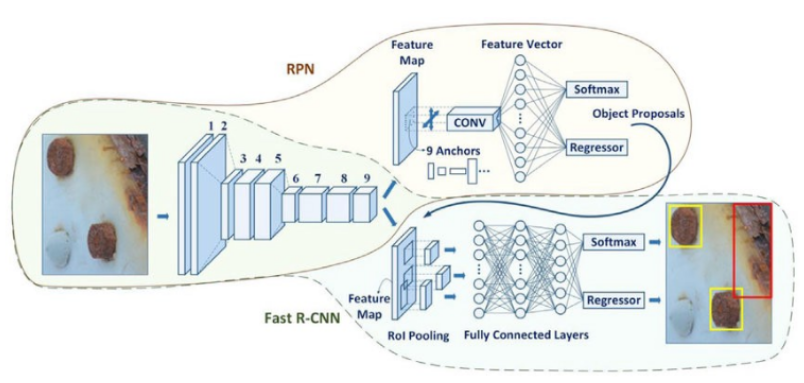
\includegraphics[width=\textwidth]{models/fasterrcnn}
    \caption{Network of Faster R-CNN}
    \label{fig:fasterrcnn1}
\end{figure}

\indent

Faster R-CNN consists of a region proposal network and a detection network which 
is improved version of Fast R-CNN as you can see in figure \ref{fig:fasterrcnn1}. 
The main improvement in Faster R-CNN is the shared convolutional layers between 
the RPN and the detection network, so that, the cost of detection is drastically 
reduced. \par

The RPN provides a simultaneous prediction of object bounds and 
objectness scores. This is done by adding two convolutional layer after the 
shared convolutional layers. The first one converts extracted feature map into a 
feature vector and the second one generates an objectness score and a regressed 
bounds for let's assume k region proposals as in figure \ref{fig:sliwinrpn1}. To 
generate region proposals, a small convolutional network slides over the shared 
feature map and each of these sliding windows are mapped to a lower-dimensional 
feature. \par

These k region proposals are fed into detection network with the extraced feature 
map from shared convolutional layers. Then, region of interest pooling extract 
region proposals from extracted feature map. Predictions are made by using this 
final feature map. Thus, RPN says the detector network where to look. \par

Training of Faster R-CNN consists of four steps. First, RPN is trained. Since 
negative samples dominate positive samples in region proposals, 256 samples are 
sampled to train RPN by using mini-batches from a single image. Then, in the 
second step, Fast R-CNN is trained separately by using the region proposals 
generated by the RPN in step 1. So far, two networks are separate and they do 
not share convolutional layers. As a step 3, the shared convolutional layers are 
held fix and RPN is fine-tuned by using detector network. As a final step, the 
layers of detection network is fine-tuned by holding the shared convolutional layers 
fixed.
\begin{figure}
    \centering
    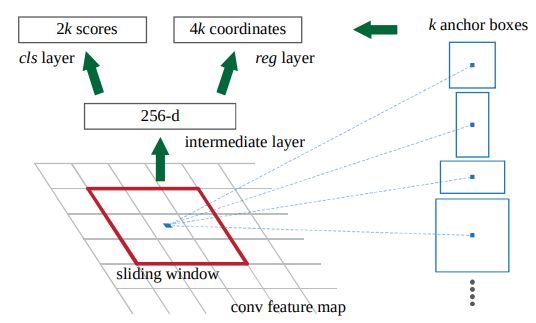
\includegraphics[width=\textwidth]{sliwinrpn}
    \caption{An example of RPN}
    \label{fig:sliwinrpn1}
\end{figure}

\end{document}